\section{Auswertung}
\label{sec:auswertung}

\subsection{Emissionsspektrum der Kupfer-Röntgenröhre}
\label{sec:auswertung:emissionsspektrum}

In \autoref{fig:emissionsspektrum} ist das Emissionsspektrum der verwendeten Röntgenröhre aufgetragen.
Hervorgehoben sind die $K_\alpha$- bzw. $K_\beta$-Kanten.
\autoref{tab:mess_emissionsspektrum} beinhaltet die zugehörigen Messwerte.

\begin{figure}
    \centering
    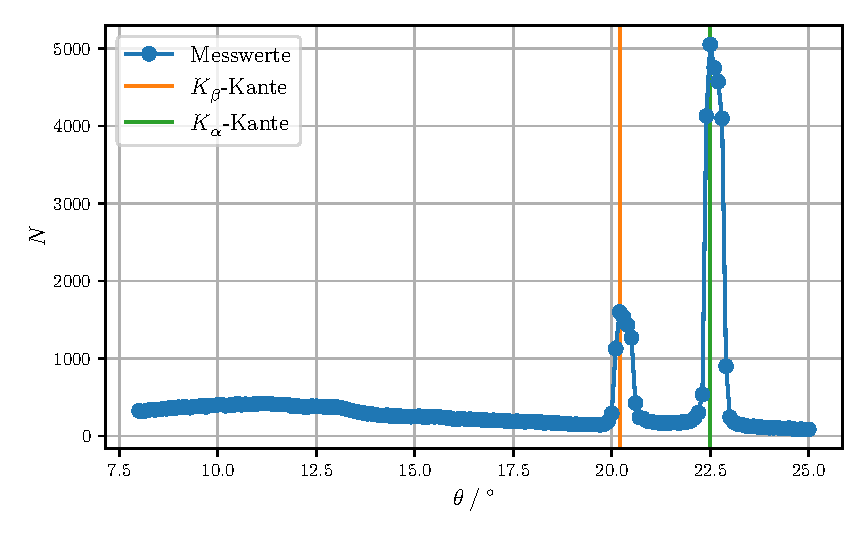
\includegraphics[width=0.9\textwidth]{build/plt/emissionsspektrum.pdf}
    \caption{Messwerte zum Emissionsspektrum der Kupfer-Röntgenröhre.}
    \label{fig:emissionsspektrum}
\end{figure}

Über den gesamten Messbereich verläuft das \hyperref[sec:theorie:bremsspektrum]{kontinuierliche Bremsspektrum}.
Zudem finden sich zwei Kanten des \hyperref[sec:theorie:char_spektrum]{charakteristischen Spektrums},
deren Intensitätsmaxima mithilfe von \texttt{scipy.signal.find\_peaks} bestimmt wurden.
Sie liegen bei
\begin{align*}
    \alpha_{K_\alpha} &= \SI{22.5}{\degree} \\
    \alpha_{K_\beta}  &= \SI{20.2}{\degree} \; .
    % identisch zu YanickKi ✓
\end{align*}

Aus der \hyperref[eqn:BraggBedingung]{Bragg-Bedingung} können nun
die Wellenlänge \hyperref[eqn:lambda_to_E]{und somit die Energie} eines Röntgenquants bestimmt werden.
Die verwendete Beziehung lautet insgesamt
\[ E = \frac{h c}{2 d \sin{\alpha}} \ . \]
Die Energien für die Peaks ergeben sich zu
\begin{align*}
    E_{K_\alpha} &= \SI{8.04}{\kilo\electronvolt} \\
    E_{K_\beta}  &= \SI{8.91}{\kilo\electronvolt} \; .
    % identisch zu YanickKi ✓
\end{align*}

\clearpage
\begin{table}
  \centering
  \caption{Messwerte zum Emissionsspektrum.}
  \label{tab:mess_emissionsspektrum}
  \begin{tabular}{
    S S[table-format=4.0] |
    S S[table-format=4.0] |
    S S[table-format=4.0] |
    S S[table-format=4.0]
    }
  \toprule
  {$\alpha \mathbin{/} \si{\degree}$} &
  {$N$} &
  {$\alpha \mathbin{/} \si{\degree}$} &
  {$N$} &
  {$\alpha \mathbin{/} \si{\degree}$} &
  {$N$} &
  {$\alpha \mathbin{/} \si{\degree}$} &
  {$N$} \\
  \midrule
  \expandableinput{build/tab/mess_emissionsspektrum_4col.tex}
  \bottomrule
  \end{tabular}
\end{table}


\FloatBarrier
\subsection{Bestimmung der Transmission als Funktion der Wellenlänge}
\label{sec:auswertung:transmission}

Die Messwerte zu diesem Abschnitt sind in \autoref{tab:mess_transmission} angegeben.
Zunächst wird eine Totzeitkorrektur nach \eqref{eqn:totzeitkorrektur} durchgeführt. % …weil?
Im Folgenden wird dann mit den angepassten Impulszahlen $I$ gerechnet.

% NOTE: Die Musterlösung sieht offenbar eine andere Fehlerrechnung vor,
% welche deutlich größere Fehler ergibt. Wir scheinen hiermit aber richtig zu liegen.
% Ich habe die √Imp-Faktoren mal weggelassen, weil sowieso [I]=Imp=1=dimensionslos ist.
% PS: Nicht von der Bezeichnung I bzw. N verwirren lassen! :)
In \autoref{fig:plt_transmission} wird die Transmission $T = \sfrac{I_\text{Al}}{I_0}$
gegen $\lambda$ aufgetragen.
Dabei wird $\lambda$ wieder mithilfe der \hyperref[eqn:BraggBedingung]{Bragg-Bedingung}
aus dem Winkel $\alpha$ gewonnen.
Die Unsicherheit der Zählrate wird bestimmt,
indem davon ausgegangen wird,
dass die \textit{Impulszahl} $I$ Poisson-verteilt ist,
also die Unsicherheit $\symup{\Delta}I = \sqrt{I}$ aufweist.
Daraus folgt für die Unsicherheit der \textit{Zählrate}
\[
  \symup{\Delta}N = \frac{\sqrt{N t}}{t}
\]
mit der Integrationszeit $t$ und $I=Nt$.

Für den \hyperref[sec:auswertung:compton_wellenlaenge]{nächsten Abschnitt} % eigentlich ein Unterabschnitt :P
wird bereits eine Regressionsrechnung durchgeführt.
Die Parameter der Ausgleichsgeraden $T = a \cdot \lambda + b$ lauten:
\begin{align*}
  a &= \SI{-0.01519(24)}{\per\pico\meter} \\
  b &= \num{1.225(14)} \ .
  % identisch zu YanickKi ✓
\end{align*}

\begin{figure}
    \centering
    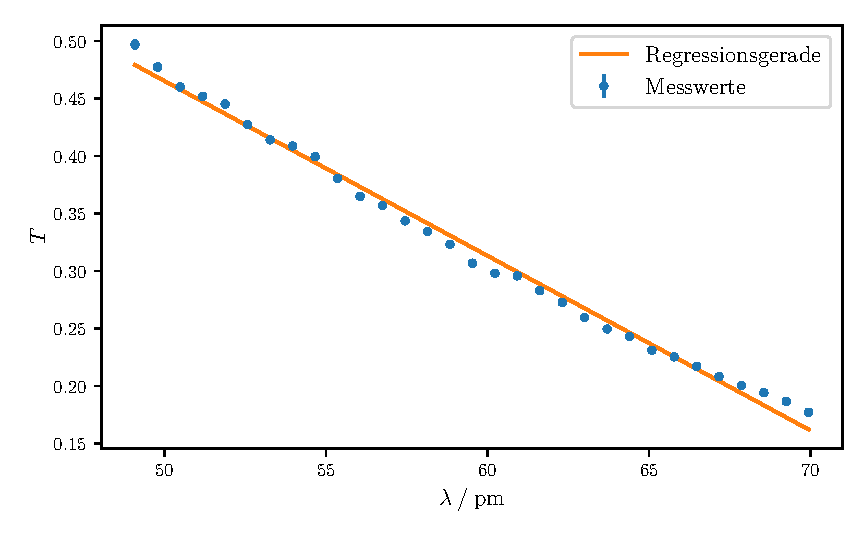
\includegraphics[width=\textwidth]{build/plt/transmission.pdf}
    \caption{Messwerte zur Transmission in Abhängigkeit der Wellenlänge.}
    \label{fig:plt_transmission}
\end{figure}

\clearpage
\begin{table}
  \centering
  \caption{Messwerte zur Transmission.}
  \label{tab:mess_transmission}
  \begin{tabular}{S S S}
  \toprule
  {$\alpha \mathbin{/} \si{\degree}$} &
  {$N_0 \mathbin{/} \si{{Imp}\per\second}$} &
  {$N_\text{Al} \mathbin{/} \si{{Imp}\per\second}$} \\
  \midrule
  \expandableinput{build/tab/mess_transmission.tex}
  \bottomrule
  \end{tabular}
\end{table}


\FloatBarrier
\subsection{Bestimmung der Compton-Wellenlänge}
\label{sec:auswertung:compton_wellenlaenge}

Es wurden die folgenden Impulszahlen über eine Integrationszeit von $t = \SI{300}{\second}$ gemessen:
\begin{align*}
  I_0 &= \SI{2731}{{Imp}} \tag {ohne Al-Absorper} \\
  I_1 &= \SI{1180}{{Imp}} \tag {mit Al-Absorber zwischen Röntgenröhre und Streuer} \\
  I_2 &= \SI{1024}{{Imp}} \tag {mit Al-Absorber zwischen Streuer und Geiger-Müller-Zählrohr}
\end{align*}
Eine Totzeitkorrektur ist hierbei nicht notwenig,
weil die resultierenden Zählraten
\begin{align*}
  N_0 &= \SI{9.10}{{Imp}\per\second} \\
  N_1 &= \SI{3.93}{{Imp}\per\second} \\
  N_2 &= \SI{3.41}{{Imp}\per\second}
\end{align*}
deutlich, genauer gesagt um den Faktor 1221,
unter der geschätzten maximalen Zählrate $\sfrac{1}{\tau} \approx \SI{11111}{{Imp}\per\second}$ liegen.
% Begründung äquivalent zu der von YanickKi ✓

Es ergeben sich Transmissionen von
\begin{align*}
  T_1 &= \frac{I_1}{I_0} = \num{0.432(15)} \\
\intertext{und}
  T_2 &= \frac{I_2}{I_0} = \num{0.375(14)} \ .
  % identisch zu YanickKi ✓
\end{align*}

Indem auf die Geradengleichung aus dem \hyperref[sec:auswertung:transmission]{vorherigen Abschnitt} zu
\[ \lambda = \frac{T-b}{a} \]
umgestellt wird,
werden die zu $T_1$ und $T_2$ gehörenden Wellenlängen
\begin{align*}
  \lambda_1 &= \SI{52.19(159)}{\pico\meter} \\
  \lambda_2 &= \SI{55.95(157)}{\pico\meter}
  % Nennwerte identisch zu YanickKi ✓
\end{align*}
bestimmt.

Daraus wird schließlich die Compton-Wellenlänge als Differenz von $\lambda_2$ und $\lambda_1$ ermittelt
(siehe \eqref{eqn:wellenlängendifferenz}):
\[ \lambda_\text{c} = \lambda_2 - \lambda_1 = \SI{3.76(114)}{\pico\meter} \ . \]
% Nennwert identisch zu BenediktSan, YanickKi ✓
% beide haben 3.76(6) 🤔
